\newpage
\section{Auswertung}
\label{sec:Auswertung}
Die in der Auswertung verwendeten Mittelwerte $n$-fach gemessener Größen sind gemäß der Gleichung
\begin{equation}
    \bar{x}=\frac{1}{n}\sum_{i=1}^n x_i.
    \label{eq:mittelwert}
\end{equation}
bestimmt. 
Die Standardabweichung des Mittelwertes ergibt sich dabei zu
\begin{equation}
    \mathup{\Delta}\bar{x}=\sqrt{\frac{1}{n(n-1)}\sum_{i=1}^n\left(x_i-\bar{x}\right)^2}.
    \label{eq:standardabweichung}
\end{equation}

Resultiert eine Größe über eine Gleichung $f$ aus N anderen fehlerbehafteten Größen $x_i$ mit $i\in\{1,…,\text{N}\}$, so
berechnet sich der Gesamtfehler $\mathup{\Delta}f(x_i)$ nach der \textsc{Gauß}schen Fehlerfortpflanzung zu
\begin{equation}
	\mathup{\Delta}f(x_1,...,x_\text{N})=\sqrt{\sum_{\text{i}=1}^\text{N}\left(\frac{\partial f}{\partial x_\text{i}}\mathup{\Delta}x_\text{i}\right)^2}.
	\label{eq:gauss_gen}
\end{equation}
% ####################################################################################################
% ####################################################################################################
% ####################################################################################################
% ####################################################################################################
% ####################################################################################################
\subsection{Eigenschaften des untersuchten Systems}
\label{sec:auswertung1}
Das untersuchte Material ist Federstahl.
Die Abmessungen des verwandten Drahtes sind in Tabelle \ref{tab:draht} aufgetragen, die Werte von Durchmesser und den Teillängen korrelieren nicht.
\begin{minipage}[t]{0.5\textwidth}
\begin{table}[H]
	\centering
	\begin{tabular}{c cc}
		\toprule
		{Durchmesser} & \multicolumn{2}{c}{Längen} \\
		{$d/\:\si{\milli\meter}$} & {$l_1/\:\si{m}$} & {$l_2/\:\si{m}$}\\
		\midrule
			0,190 & 0,551 & 0,500 \\
			0,189 & 0,551 & 0,510 \\
			0,191 & 0,550 & 0,500 \\
			0,193 & 0,551 & 0,520 \\
			0,195 & 0,551 & 0,520 \\
		\bottomrule
	\end{tabular}
	\caption{Abmessungen des Drahtes.}
	\label{tab:draht}
\end{table}
\end{minipage}
\begin{minipage}[t]{0.5\textwidth}
\begin{table}[H]
	\centering
	\begin{tabular}{cc}
		\toprule
		{Masse der Kugel} & {Radius der Kugel} \\
		{$m_K/\:\si{\gram}$} & {$r_K/\:\si{\milli\meter}$}\\
		\midrule
			$\SI{512.20(20)}{}$& $\SI{25.3800(18)}{}$\\
		\bottomrule
	\end{tabular}
	\caption{Eigenschaften der Kugel.}
	\label{tab:kugel}
\end{table}
\end{minipage}
Für die folgenden Rechnungen wird der Durchmesser $d=\SI{0.1916(11)}{\milli\meter}$ und die Gesamtlänge $l=\SI{0.6018(5)}{\meter}$ benutzt.
\newpage
Die Eigenschaften der Kugel sind in Tabelle \ref{tab:kugel} aufgetragen.
Zur Berücksichtigung des Trägheitsmomentes der Kugelaufhängung $\Theta_\text{Aufhängung}$ wird das Kugelträgheitsmoment $\Theta_\text{Kugel}$ in den folgenden Rechnungen mit dem Gesamttägheitsmoment $\Theta$ des schwingenden Systems ersetzt.
Mit 
\begin{alignat}{3}
	\Theta	&=\Theta_\text{Kugel} &&+\Theta_\text{Aufhängung}\label{eq:gesamttraegheit}\\ 
		&=\frac{2}{5} m_\text{K} r_\text{K}^2 &&+\SI{22.5e-7}{\kilo\gram\meter\squared}
\end{alignat}
wird das Gesamtträgheitsmoment $\Theta=\SI{0.13422(6)e-3}{\kilo\gram\meter\squared}$ angenommen.
% ####################################################################################################
% ####################################################################################################
% ####################################################################################################
% ####################################################################################################
% ####################################################################################################
\subsection{Bestimmung des Schubmodules \texorpdfstring{$G$}{G}}
\begin{table}
	\centering
	\begin{tabular}{c}
	\toprule
	{$T_G/\:\si{\second}$}\\
	\midrule
18,585\\
18,598\\
18,593\\
18,588\\
18,585\\
18,588\\
18,589\\
18,592\\
18,594\\
18,594\\
18,598\\
{Bitte berichtigen!}\\
	\bottomrule
	\end{tabular}
	\caption{Schwingungsdauern zur Berechnung des Schubmoduls $G$.}
	\label{tab:T_G}
\end{table}
Die zur Berechnung des Schubmoduls $G$ benötigeten Schwingdauern $T_\text{G}$ sind in Tabelle \ref{tab:T_G} aufgetragen.
Der Schubmodul $G$ wird mittels der Formel \eqref{eq:G} berechnet.
Es gilt
\begin{align}
	G 	&=  8 \Theta\frac{\pi L}{T^2 r_D^4}\\% = \frac{16}{5} \frac{(\pi m_K r_K^2 L)}{(T^2 r_D^4)} 
		&=	\SI{69.7\pm1.6}{\giga\newton\per\meter\squared}
	\label{eq:schubmodul}
	\end{align}
Aus der Literatur ist der Schubmodul für das Material Federstahl mit
\begin{equation}
	G_\text{Theorie} = \SI{73.575}{\giga\newton\per\meter\squared}
\end{equation}bekannt.
Die Messung weicht von der Theorie um $-5.27\%$ ab.
% ####################################################################################################
% ####################################################################################################
% ####################################################################################################
% ####################################################################################################
% ####################################################################################################
\subsection{Bestimmung des Dipolmomentes \texorpdfstring{$m$}{m}}
\label{sec:auswertung2}
Tabelle \ref{tab:T_m} zeigt in Abhängigkeit von der Stromstärke $I$ der \textsc{Helmholtz}-Spule die gemessenen Schwingdauern $T_{m,i}$ sowie deren Mittelwerte und Standardabweichungen. 
Die einzelnen Schwingdauern verschiedener Stromstärken $I$ korrelieren nicht.
\begin{table}[ht]
	\centering
	\begin{tabular}{l|ccccc}
	\toprule
{$I/\:\si{\ampere}$} & 0,1 & 0,2 & 0,4 & 0,6 & 0,8\\
	\midrule
{$T_{m,i}/\:\si{\second}$}	& 11,424 &  9,526 &  6,889 &  5,837 &  5,171 \\
						& 11,441 &  9,513 &  6,949 &  5,785 &  5,169 \\
						& 11,386 &  9,490 &  6,953 &  5,841 &  5,172 \\
						& 11,411 &  9,480 &  6,955 &  5,831 &  5,162 \\
						& 11,384 &  9,473 &  6,954 &  5,844 &  5,162 \\
	\bottomrule
{$T_m/\:\si{\second}$}	& \SI{11.41(1)}{} & \SI{9.49(1)}{} & \SI{6.94(1)}{} & \SI{5.83(1)}{} & \SI{5.17(1)}{} \\
	\end{tabular}
	\caption{Schwingungsdauern zur Berechnung des magnetischen Moments $m$.}
	\label{tab:T_m}
\end{table}
Zur Bestimmung des Dipolmomentes wird die Gleichung \eqref{eq:schwingdauer_magnet} benutzt, um die Magnetfeldstärke $B$ 
der \textsc{Helmholtz}-Spule gegen das reziproke Schwingdauer-Quadrat $\frac{1}{T_{m}^2}$ aufzutragen.
Die Magnetfeldstärke $B$ der \textsc{Helmholtz}-Spule ist durch die Gleichung \eqref{eq:B_HS} und durch den Spulenstrom $I$ bekannt.
Mit der Linearisierung
\begin{equation}
	B = \underbrace{4\pi^2\frac{\Theta}{m}}_{a_\text{lin}} \underbrace{\frac{1}{T_m^2}}_{x_\text{lin}} - \underbrace{\frac{D}{m}}_{b_\text{lin}}
	\label{eq:B_lin}
\end{equation}
und der Regression mittels der Formeln \eqref{eq:regress}
sind die Parameter des Fits
\begin{align}
	a_\text{lin}&=	\SI{0.1036(22)}{\tesla\second\squared}, \\
	b_\text{lin}&=	-\SI{3.16(53)e-04}{\tesla}.
\end{align}
\begin{figure}[p]
	\centering
	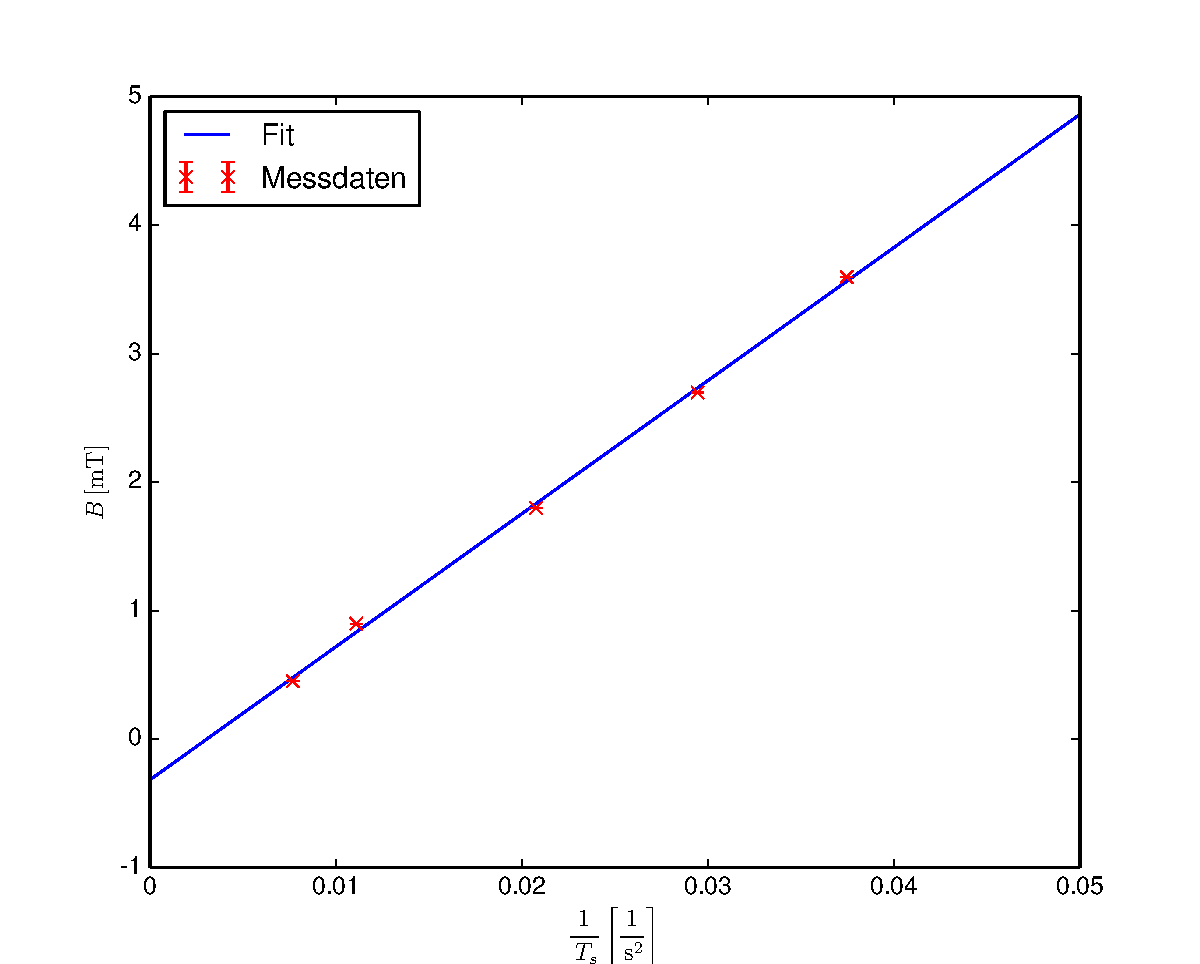
\includegraphics[width=0.7\textwidth]{Bilder/Magnetfeld.pdf}
	\caption{Messdaten und Regression der Schwingdauern $T_\text{S}$ und der Magnetfeldstärke $B$.}
	\label{fig:Magnetfeld}
\end{figure}
Es folgt für das magnetische Moment
\begin{align}
	m 	&= 4\pi^2\frac{\Theta}{a_\text{lin}}\\
		&= \SI{0.0512(11)}{\tesla\meter}
	\label{eq:Magnetmoment_lin}
\end{align}
% ####################################################################################################
% ####################################################################################################
% ####################################################################################################
% ####################################################################################################
% ####################################################################################################
\subsection{Bestimmung der \texorpdfstring{Erdmagnetfeldstärke $B_\text{Erde}$}{Magnetfeldstärke B der Erde}}
\label{sec:auswertung3}
\begin{table}
	\centering
	\begin{tabular}{c}
	\toprule
	{$T_G/\:\si{\second}$}\\
	\midrule
18,413\\
18,411\\
18,390\\
18,409\\
18,379\\
18,404\\
18,395\\
18,399\\
18,396\\
18,391\\
	\bottomrule
	\end{tabular}
	\caption{Schwingungsdauern zur Berechnung des Schubmoduls $G$.}
	\label{tab:T_G}
\end{table}
Die gemessenen Zeiten $T_{\text{E},i}$ sind in Tabelle \ref{tab:T_E} aufgetragen, der Mittelwert mit Standardabweichung ist
$T_\text{E}=\SI{18.3987(34)}{\second}$.\newpage
Mithilfe der Gleichung \eqref{eq:B_lin} wird die Stärke des Erdmagnetfeldes $B_\text{Erde}$ bestimmt.
Aus Abschnitt \ref{sec:Theorie}, Gleichung \eqref{eq:Richtgrosse} und Abschnitt \ref{sec:auswertung2}, Gleichung \eqref{eq:Magnetmoment_lin} sind die in Formel \eqref{eq:B_lin} benötigten Größen $m$ und $D$ bekannt.\\
Die Winkelrichtgröße $D$ beträgt
$D = \SI{1.5333(7)e-05}{\newton\meter}$.
Damit ist die Stärke des Erdmagnetfeldes
\begin{equation}
	B_\text{Erde}=\SI{6.27(18)e-06}{\tesla}.
\end{equation}
\begin{figure}[p]
\centering
\begin{subequations}
	\begin{equation}
		\Delta = N \sum{x^2} - {\biggl(\sum{x}\biggr)}^2
	\end{equation}
	\begin{equation}
		a_{\text{Reg}} = \frac{N\sum{x\cdot y} - \sum{x} \cdot \sum{y}}{\Delta}
	\end{equation}
    \begin{equation}
		b_{\text{Reg}} = \frac{\sum{x^2} \cdot \sum{y} - \sum{x} \cdot \sum{x \cdot y}}{\Delta}
	\end{equation}
	\begin{equation}
		\sigma_{y} = \sqrt{\frac{\sum{(y - a_{\text{Reg}} \cdot x - b_{\text{Reg}})^2}}{N - 2}}
	\end{equation}
	\begin{equation}
		\sigma_{a} = \sigma_{y} \sqrt{\frac{N}{\Delta}}
	\end{equation}
	\begin{equation}
		\sigma_{b} = \sigma_{y} \sqrt{\frac{\sum{x^2}}{\Delta}}
	\end{equation}
	(vgl. \cite{scipy})
	mit $x=x_\text{lin}=\frac{1}{T_m^2}$, $y=B$, $a_\text{Reg}=a_\text{lin}$, $b_\text{Reg}=b_\text{lin}$ und der Anzahl der Datenpaare N 
	\label{eq:regress}
\end{subequations}
\end{figure}
% ####################################################################################################
% ####################################################################################################
% ####################################################################################################
% ####################################################################################################
% ####################################################################################################
\subsection{Bestimmung der \texorpdfstring{\textsc{Poisson}schen Querkontraktionszahl $\mu$}{Poissonschen Querkontraktionszahl} und des Kompressionsmoduls \texorpdfstring{$Q$}{Q}}
\label{sec:auswertung4}
Der Literaturwert des Elastizitätsmoduls $E$ für Federstahl ist
\begin{equation}
	E = \SI{190,3}{\giga\pascal},
\end{equation}
aus Abschnitt \ref{sec:auswertung1}, Gleichung \eqref{eq:schubmodul} ist der Schubmodul $G$ mit
\begin{equation}
	G=	\SI{69.7\pm1.6}{\giga\newton\per\meter\squared}
\end{equation}
bekannt.
Mithilfe der Zusammenhänge nach Gleichung \eqref{eq:modulbeziehungen} gilt für die \textsc{Poisson}sche Querkontraktionszahl $\mu$ und für den Kompressionsmodul $Q$
\begin{align}
	\mu &= \frac{E}{2G}-1 & Q 	&= \frac{E}{3(1-2\mu)}\\
		&= \SI{0.362(31)}{}.& &= \SI{0.23(5)}{\tera\newton\per\meter}
	\label{eq:mu}
\end{align}
% 73,575 und 190,3